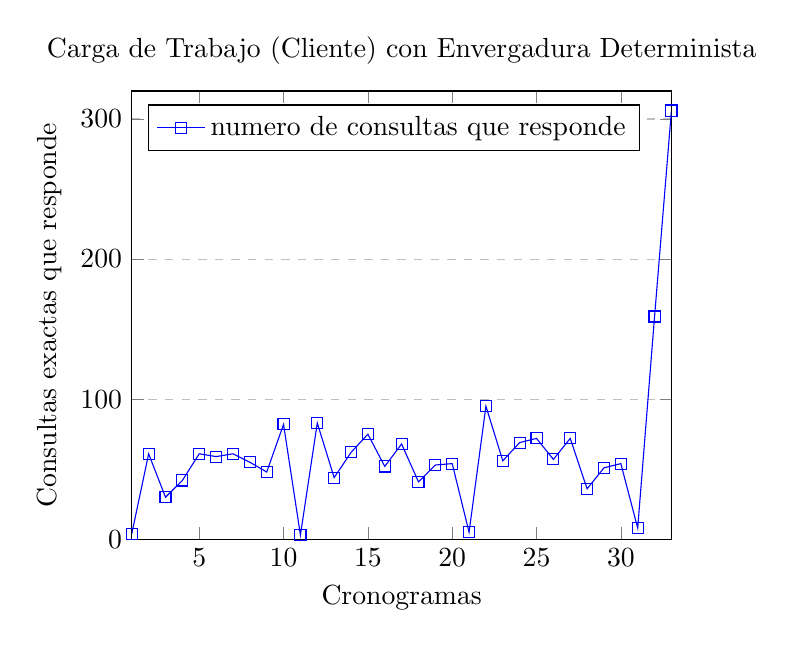
\begin{tikzpicture}
\begin{axis}[
    title={Carga de Trabajo (Cliente) con Envergadura Determinista},
    xlabel={Cronogramas},
    ylabel={Consultas exactas que responde},
    xmin=1, xmax=33,
    ymin=0, ymax=320,
    xtick={},
    ytick={},
    legend pos=north west,
    ymajorgrids=true,
    grid style=dashed,
]

\addplot[
    color=blue,
    mark=square,
    ]
    coordinates {
    %CARGA DE TRABAJO CLIENTE
        (1,4)
        (2,61)
        (3,30)
        (4,42)
        (5,61)
        (6,59)
        (7,61)
        (8,55)
        (9,48)
        (10,82)
        (11,3)
        (12,83)
        (13,44)
        (14,62)
        (15,75)
        (16,52)
        (17,68)
        (18,41)
        (19,53)
        (20,54)
        (21,5)
        (22,95)
        (23,56)
        (24,69)
        (25,72)
        (26,57)
        (27,72)
        (28,36)
        (29,51)
        (30,54)
        (31,8)
        (32,159)
        (33,306)
    };
    \legend{numero de consultas que responde}

\end{axis}
\end{tikzpicture}



